This section provides an overview of the experimental setup. It includes an examination of the limited in-domain dataset, available to study during this project, the ImageNet dataset used to pre-train the general-domain model, and the Places365 dataset used to pre-train the in-domain model,
\subsection{Danish Real Estate 2019 Data (DRE19)}\label{sec:DRE19}
This dataset was collected and catalogued by \textbf{\textit{Ingwersen}}\autocite{Ingwersen} and the author using web crawlers targeting various danish real estate websites.
The entire dataset consists of 21000 unique images, however only \textbf{6415} have been labeled. For training the remaining part of the dataset, an unsupervised method like the one proposed in \autoref{sec:contrastive}, should be considered for future work.
\begin{figure}[H]
    \centering
    \begin{subfigure}[b]{0.3\textwidth}
      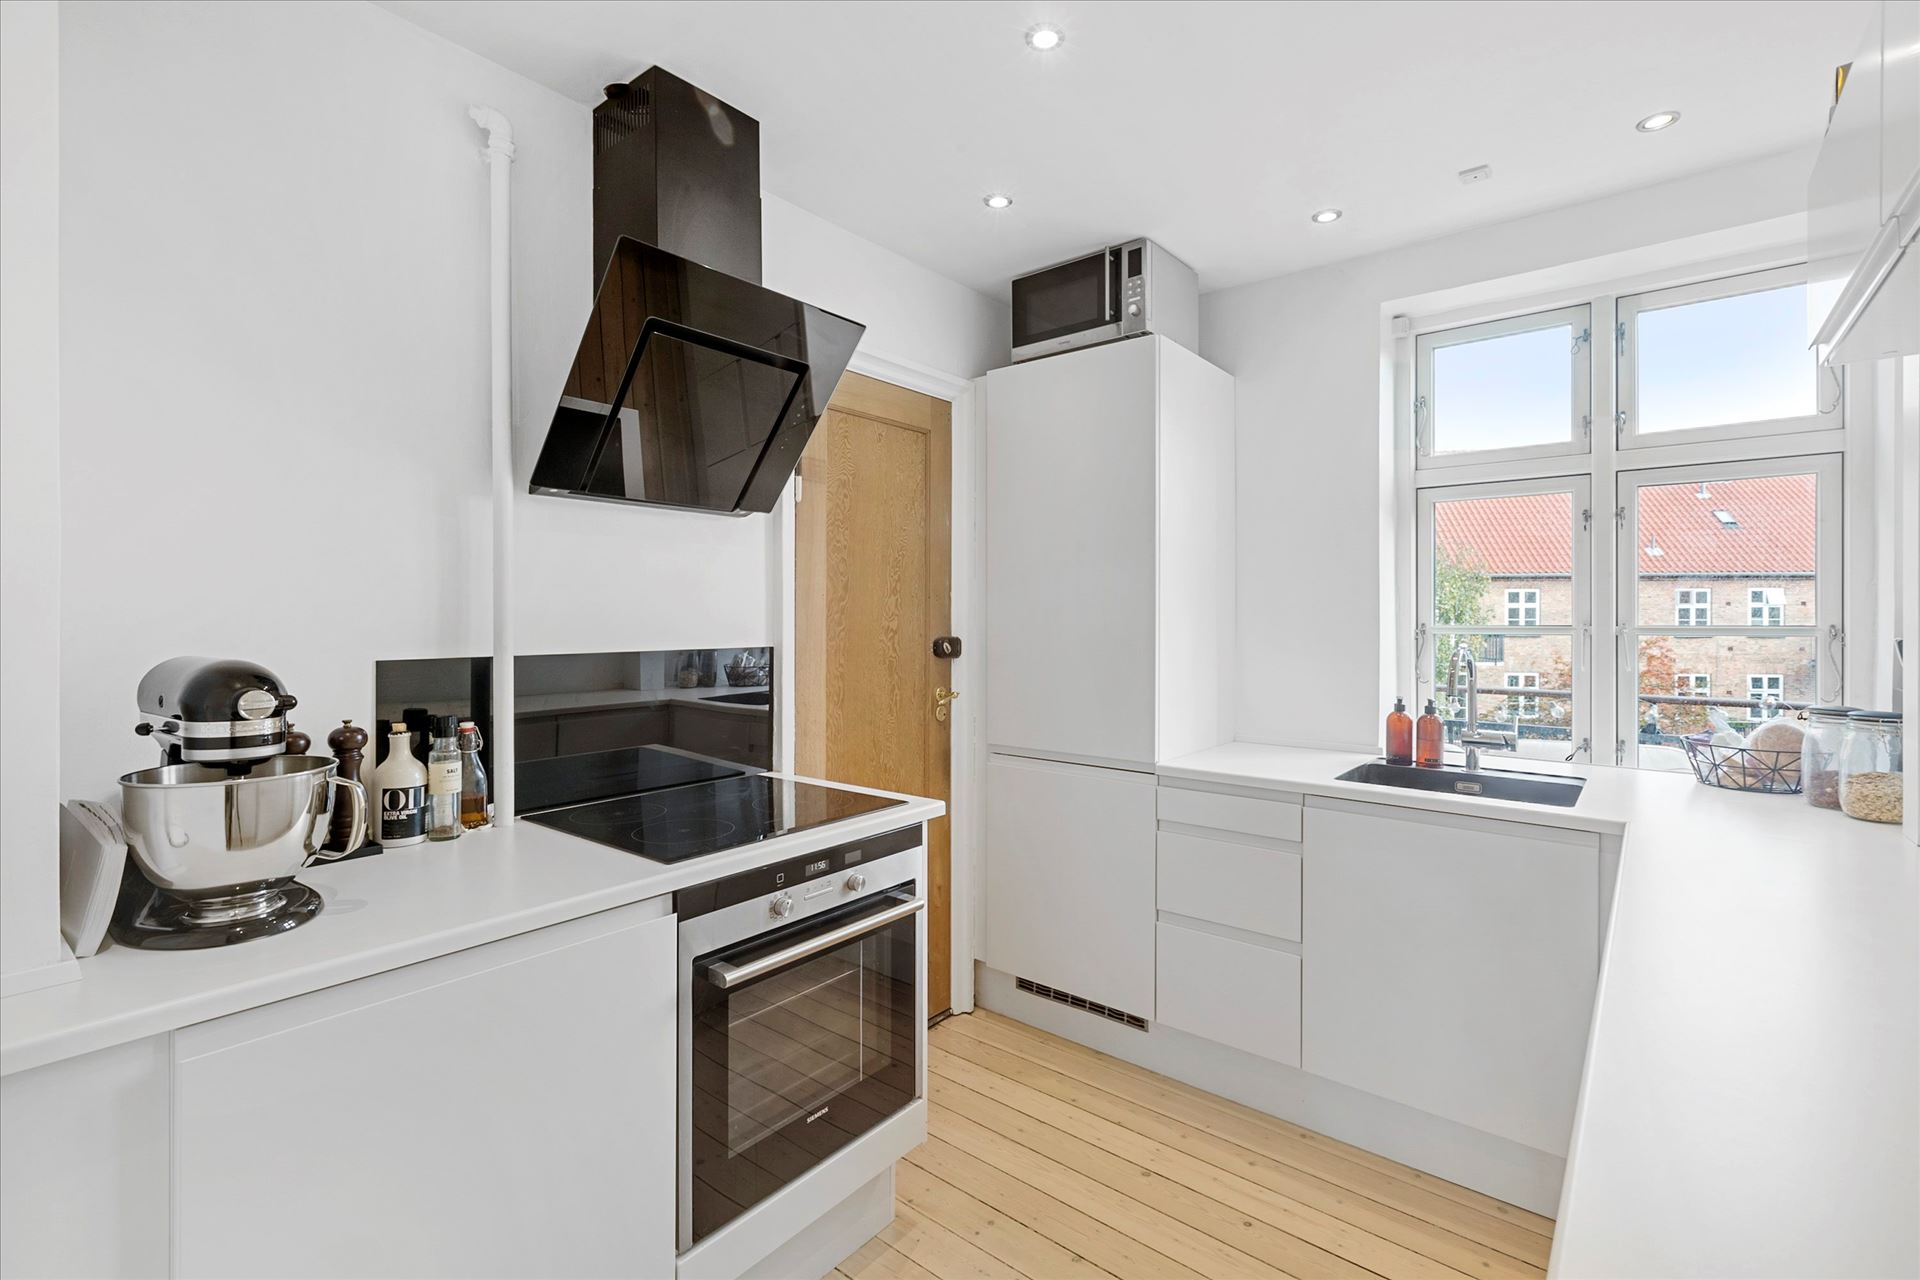
\includegraphics[width=\textwidth]{pictures/random/kitchen}
      \caption{Label: Kitchen}
      \label{fig:1}
    \end{subfigure}
    %
    \begin{subfigure}[b]{0.3\textwidth}
      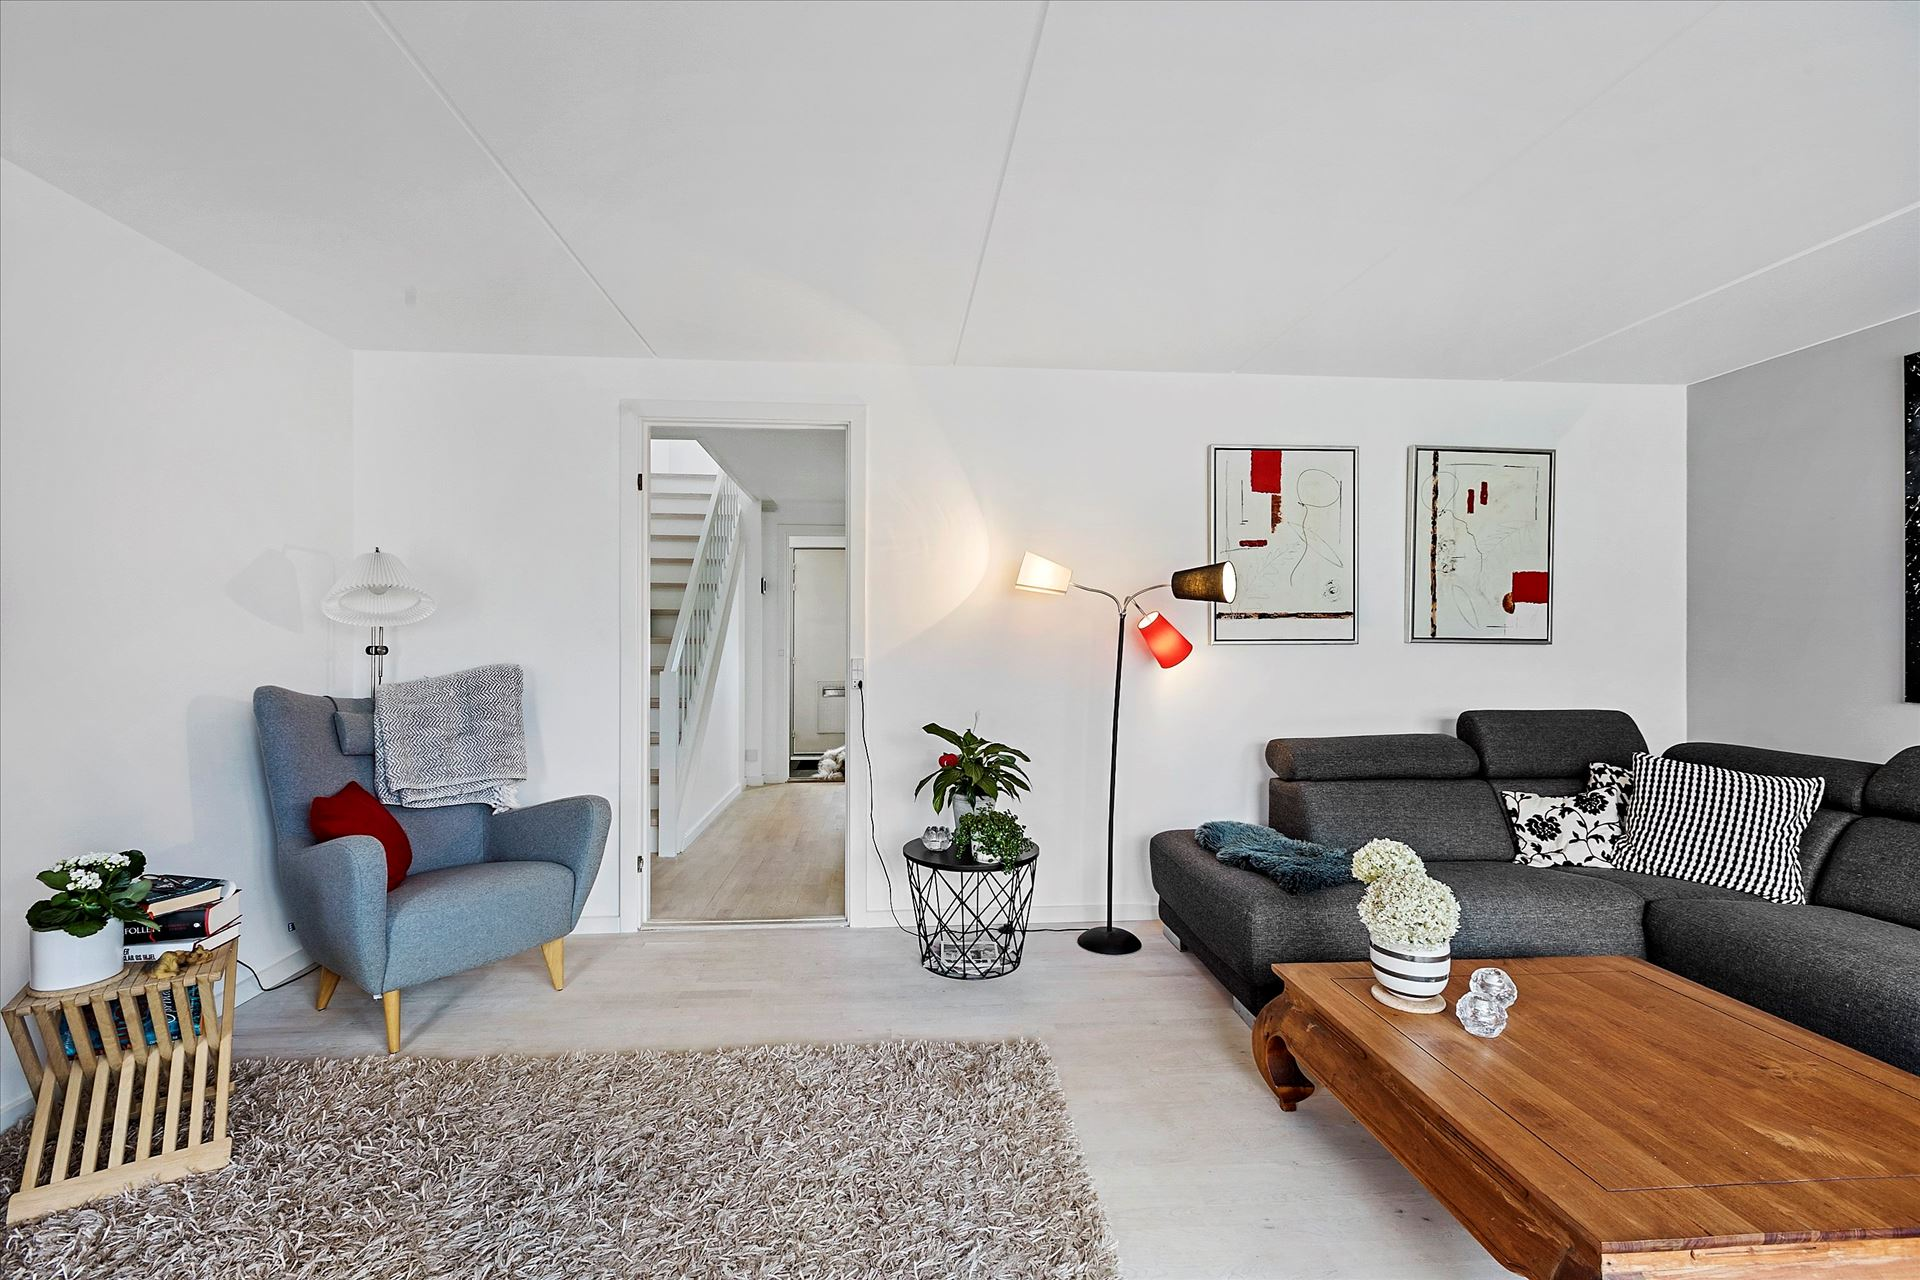
\includegraphics[width=\textwidth]{pictures/random/livingroom}
      \caption{Label: Living Room}
      \label{fig:2}
    \end{subfigure}
    %
    \begin{subfigure}[b]{0.3\textwidth}
      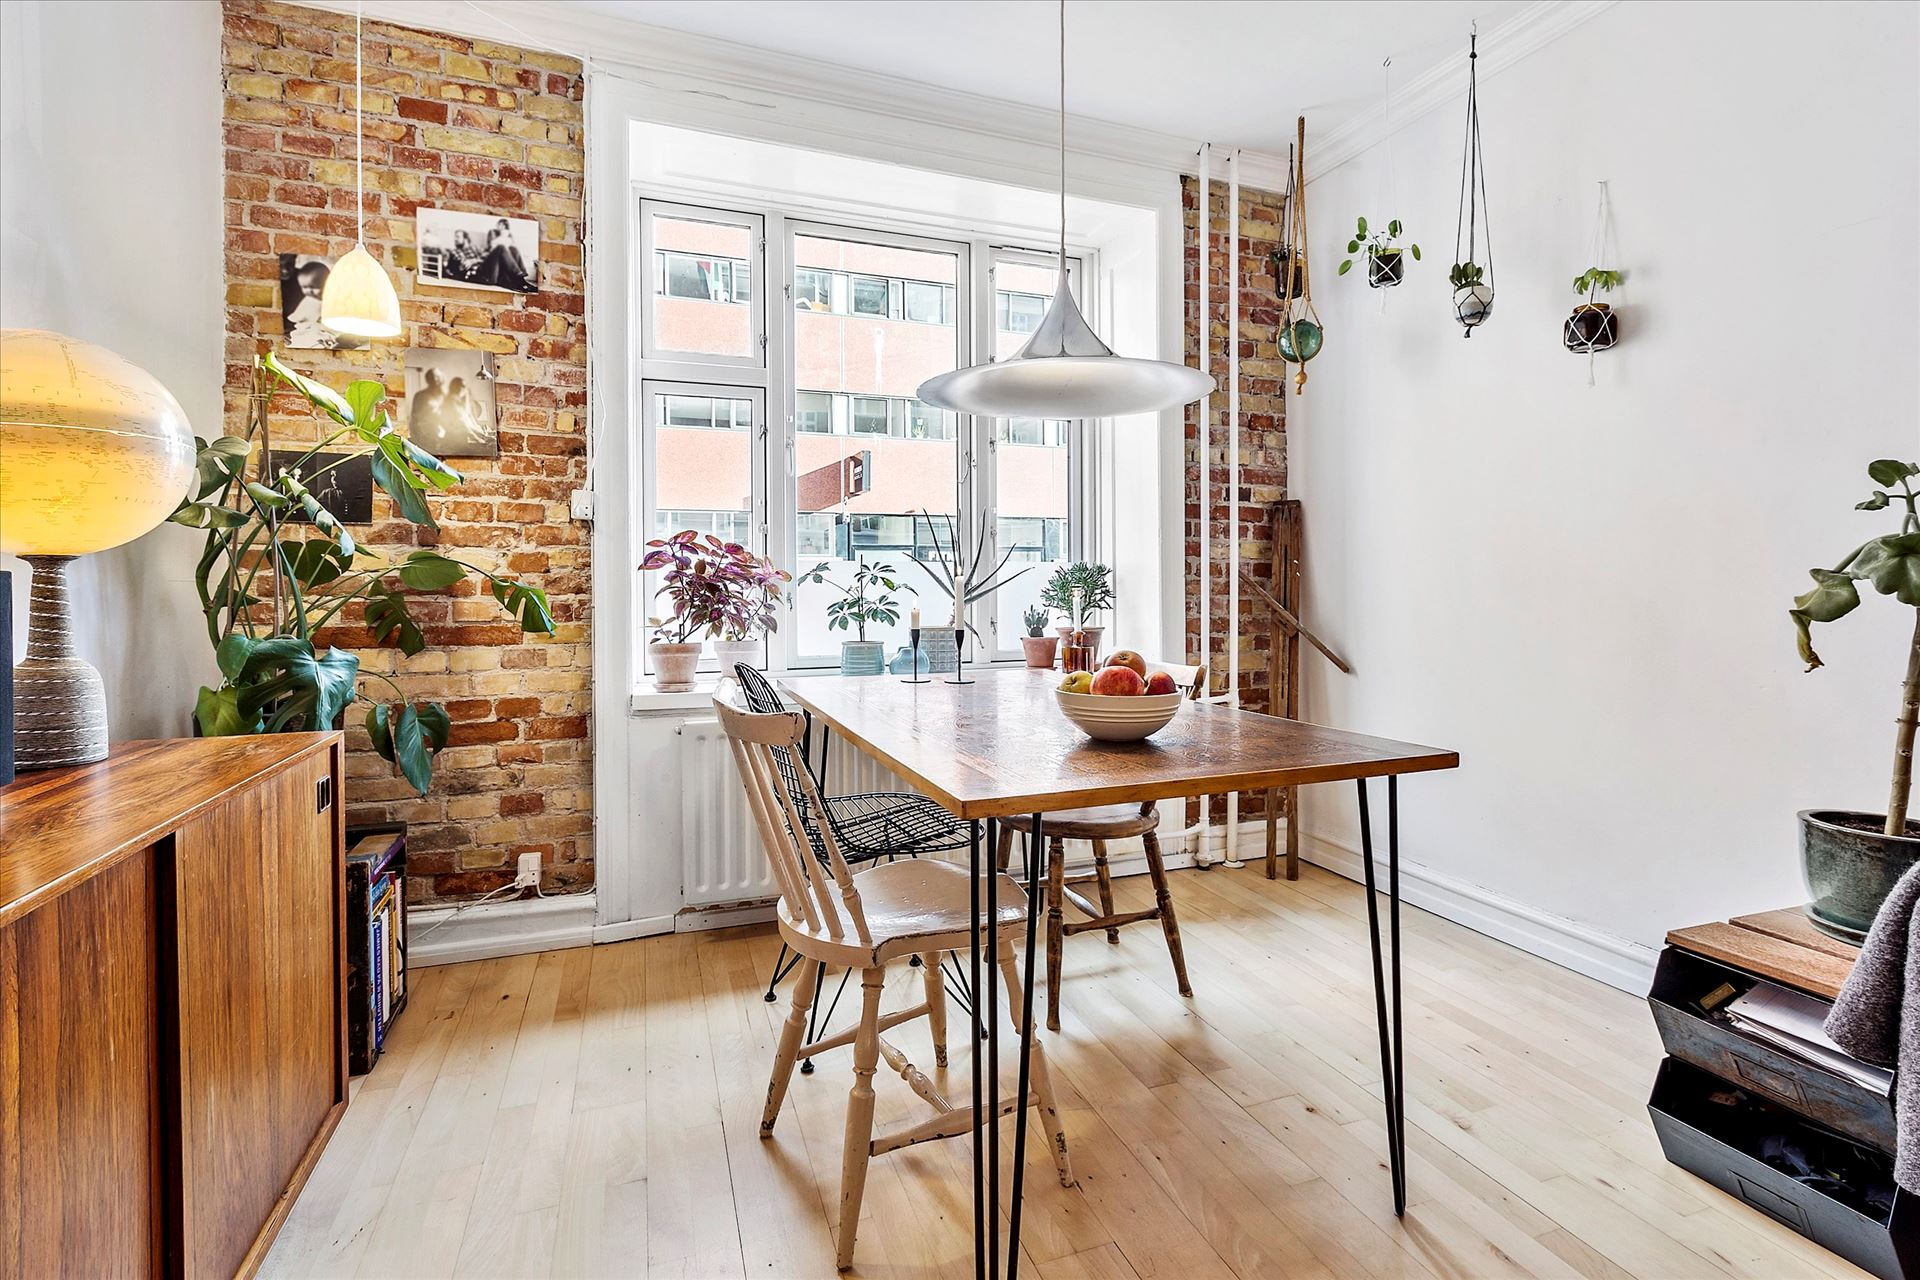
\includegraphics[width=\textwidth]{pictures/random/diningroom}
      \caption{Label: Dining Room}
      \label{fig:3}
    \end{subfigure}
    %
    \begin{subfigure}[b]{0.3\textwidth}
      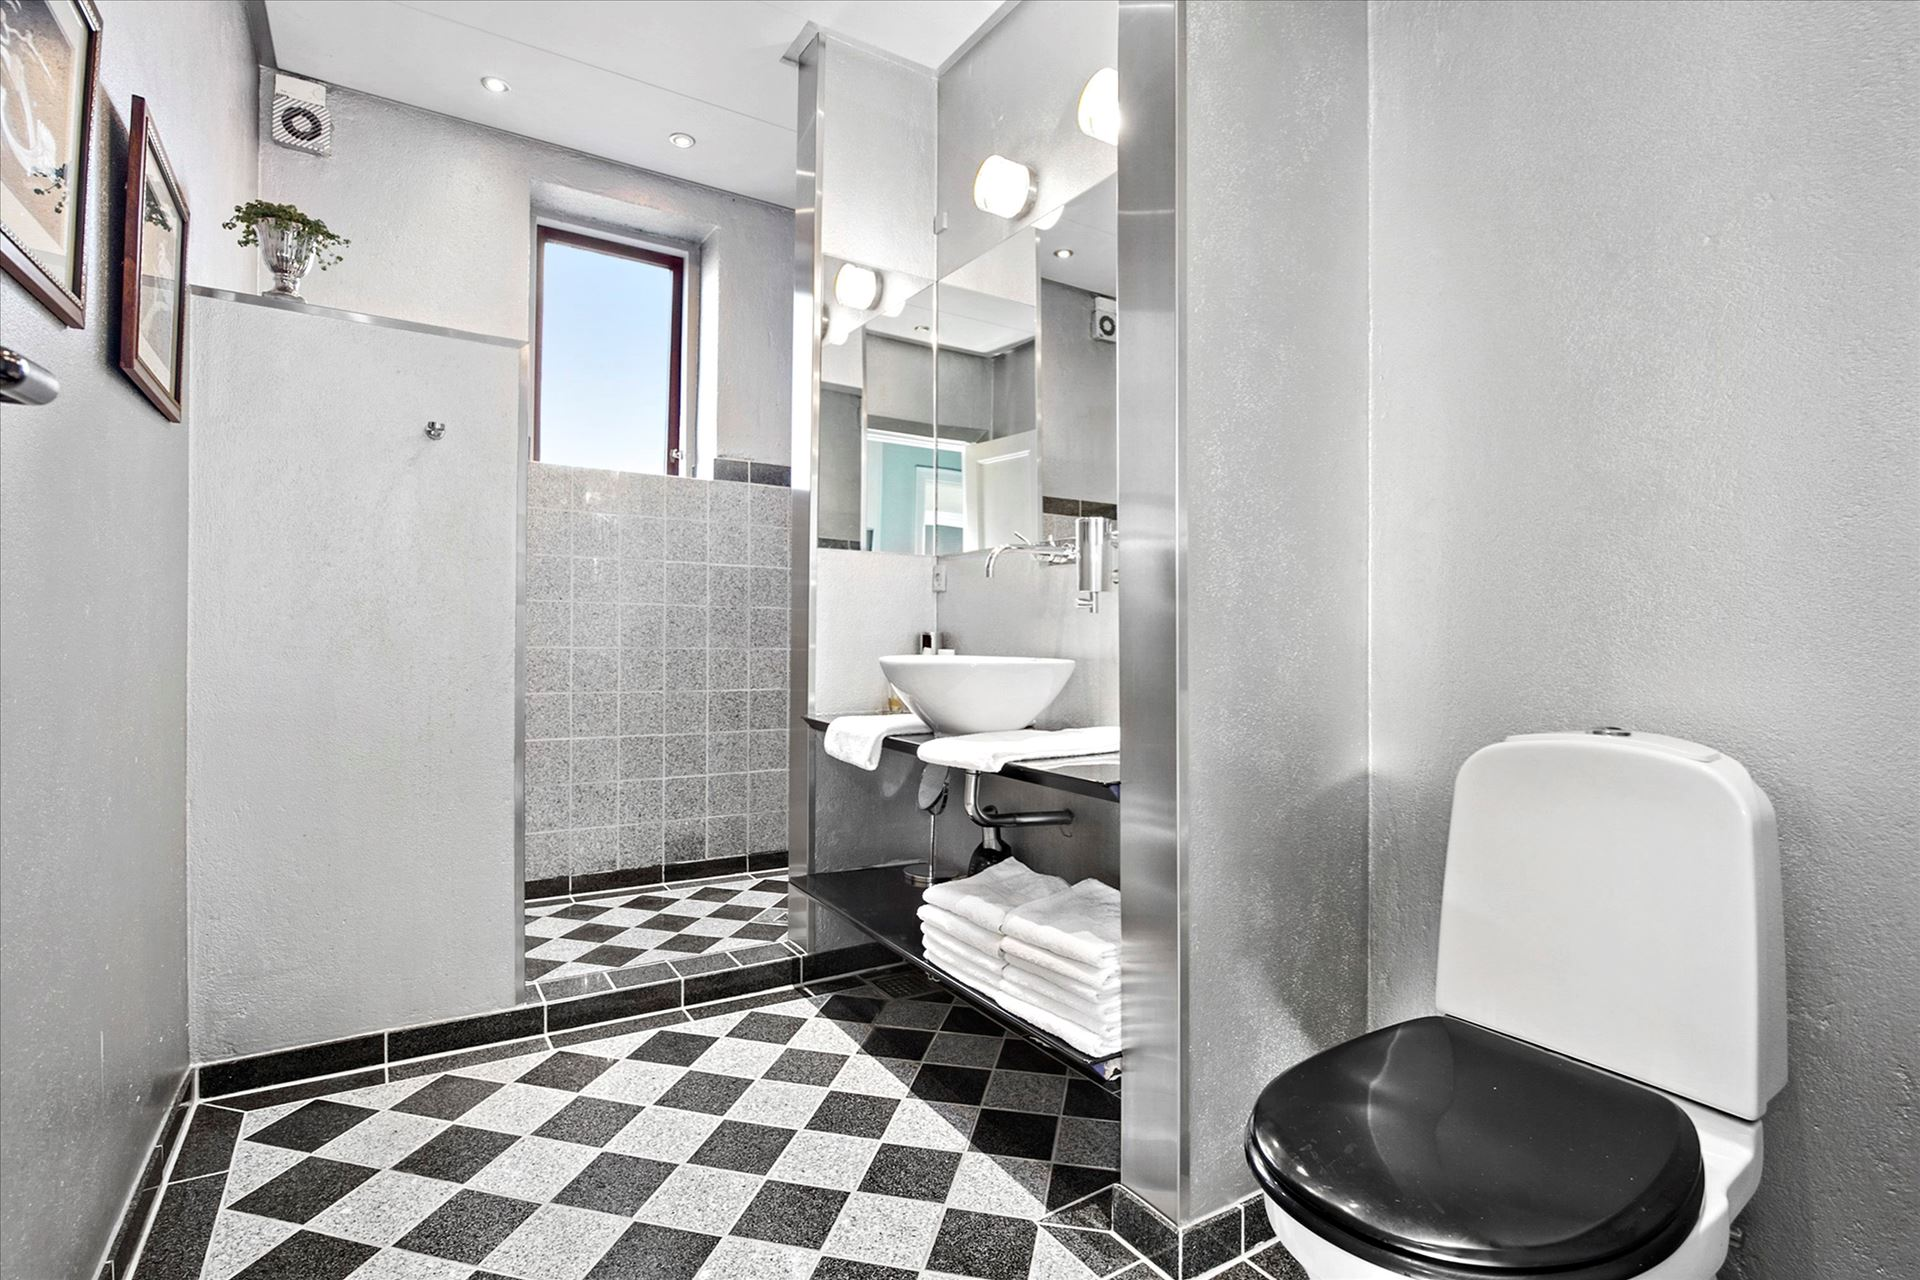
\includegraphics[width=\textwidth]{pictures/random/bathroom}
      \caption{Label: Bathroom}
      \label{fig:4}
    \end{subfigure}
    \begin{subfigure}[b]{0.3\textwidth}
      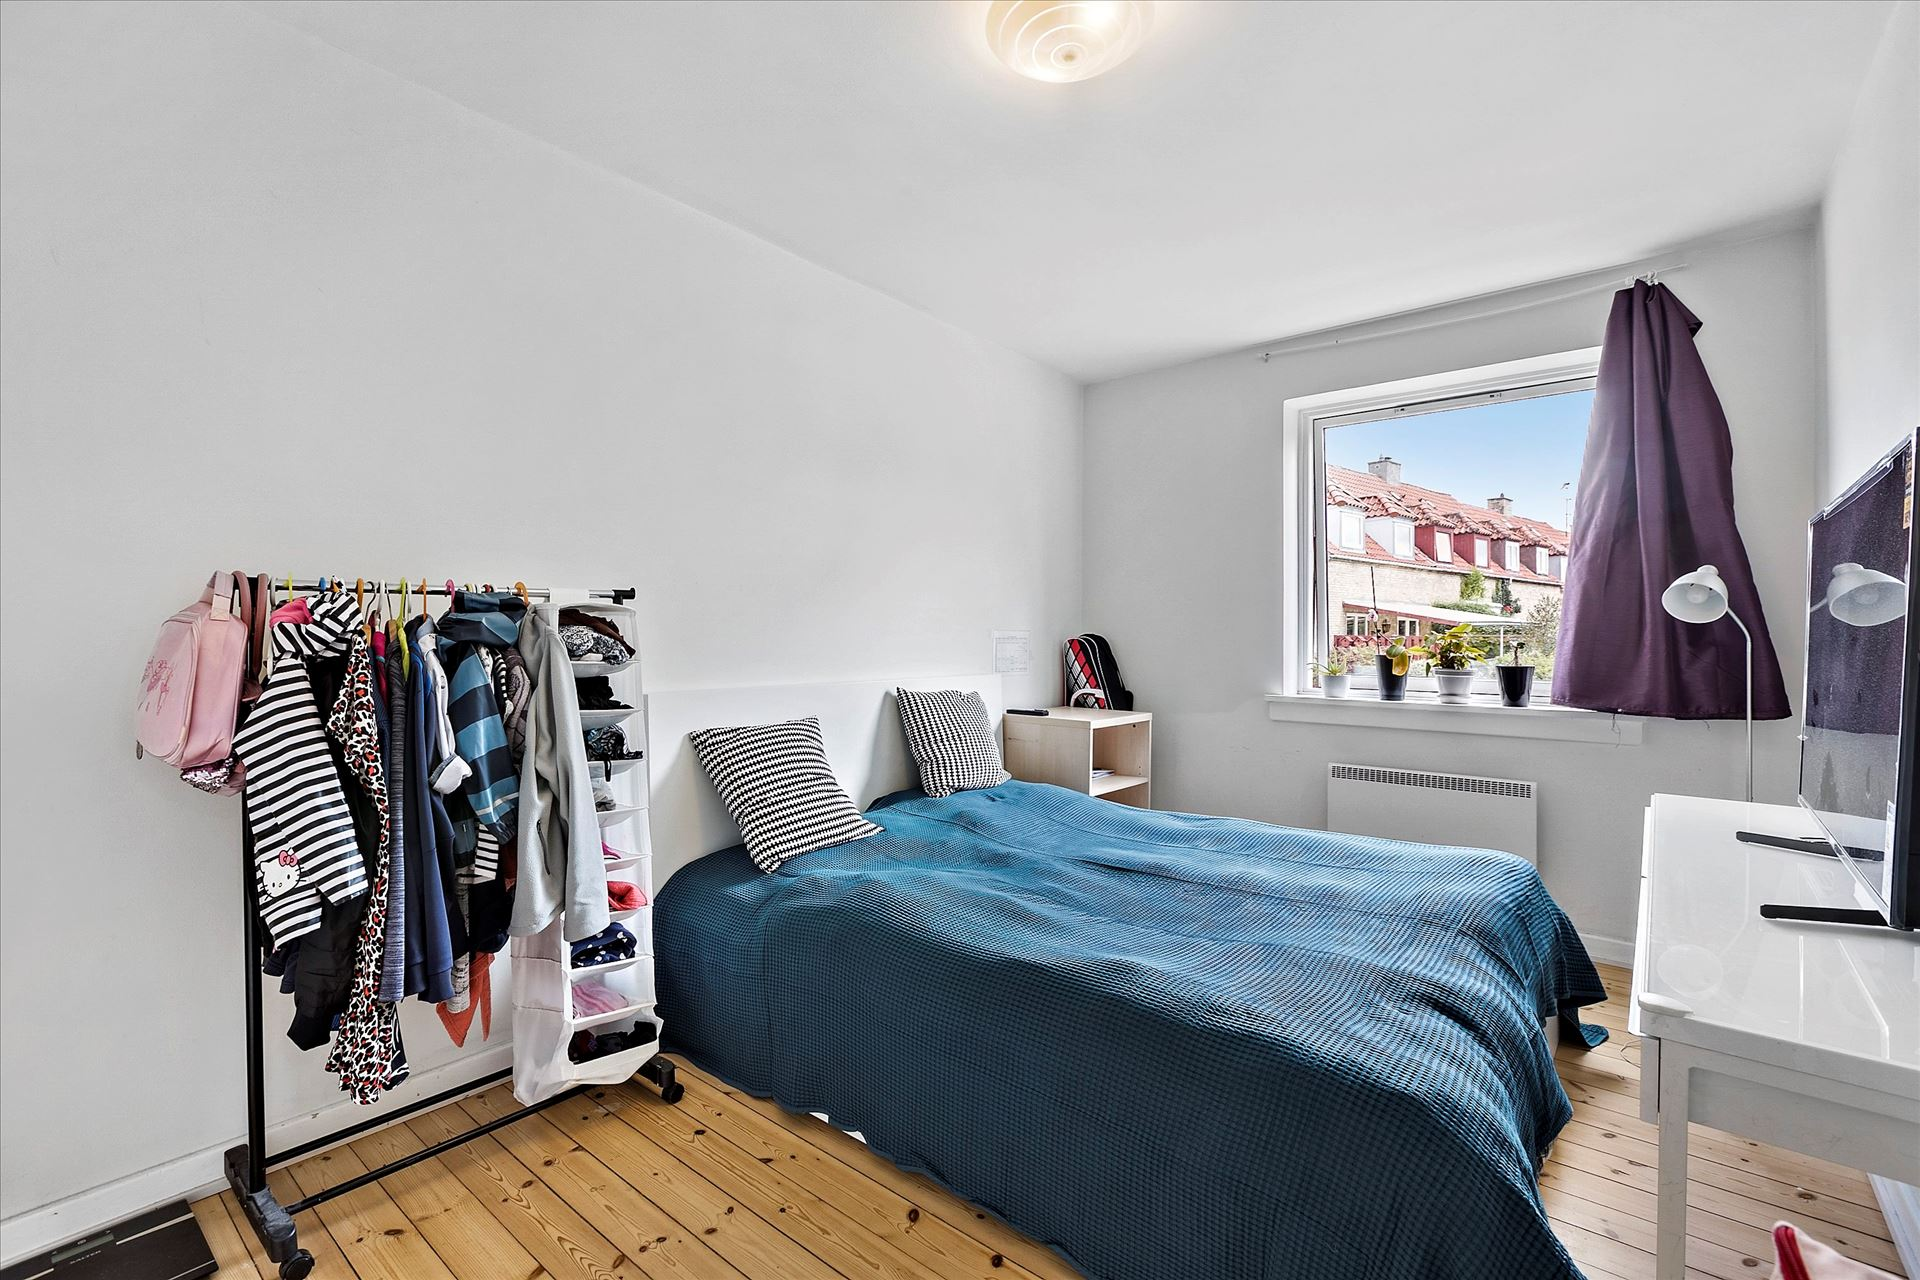
\includegraphics[width=\textwidth]{pictures/random/bedroom}
      \caption{Label: Bedroom}
      \label{fig:4}
    \end{subfigure}
    \begin{subfigure}[b]{0.3\textwidth}
      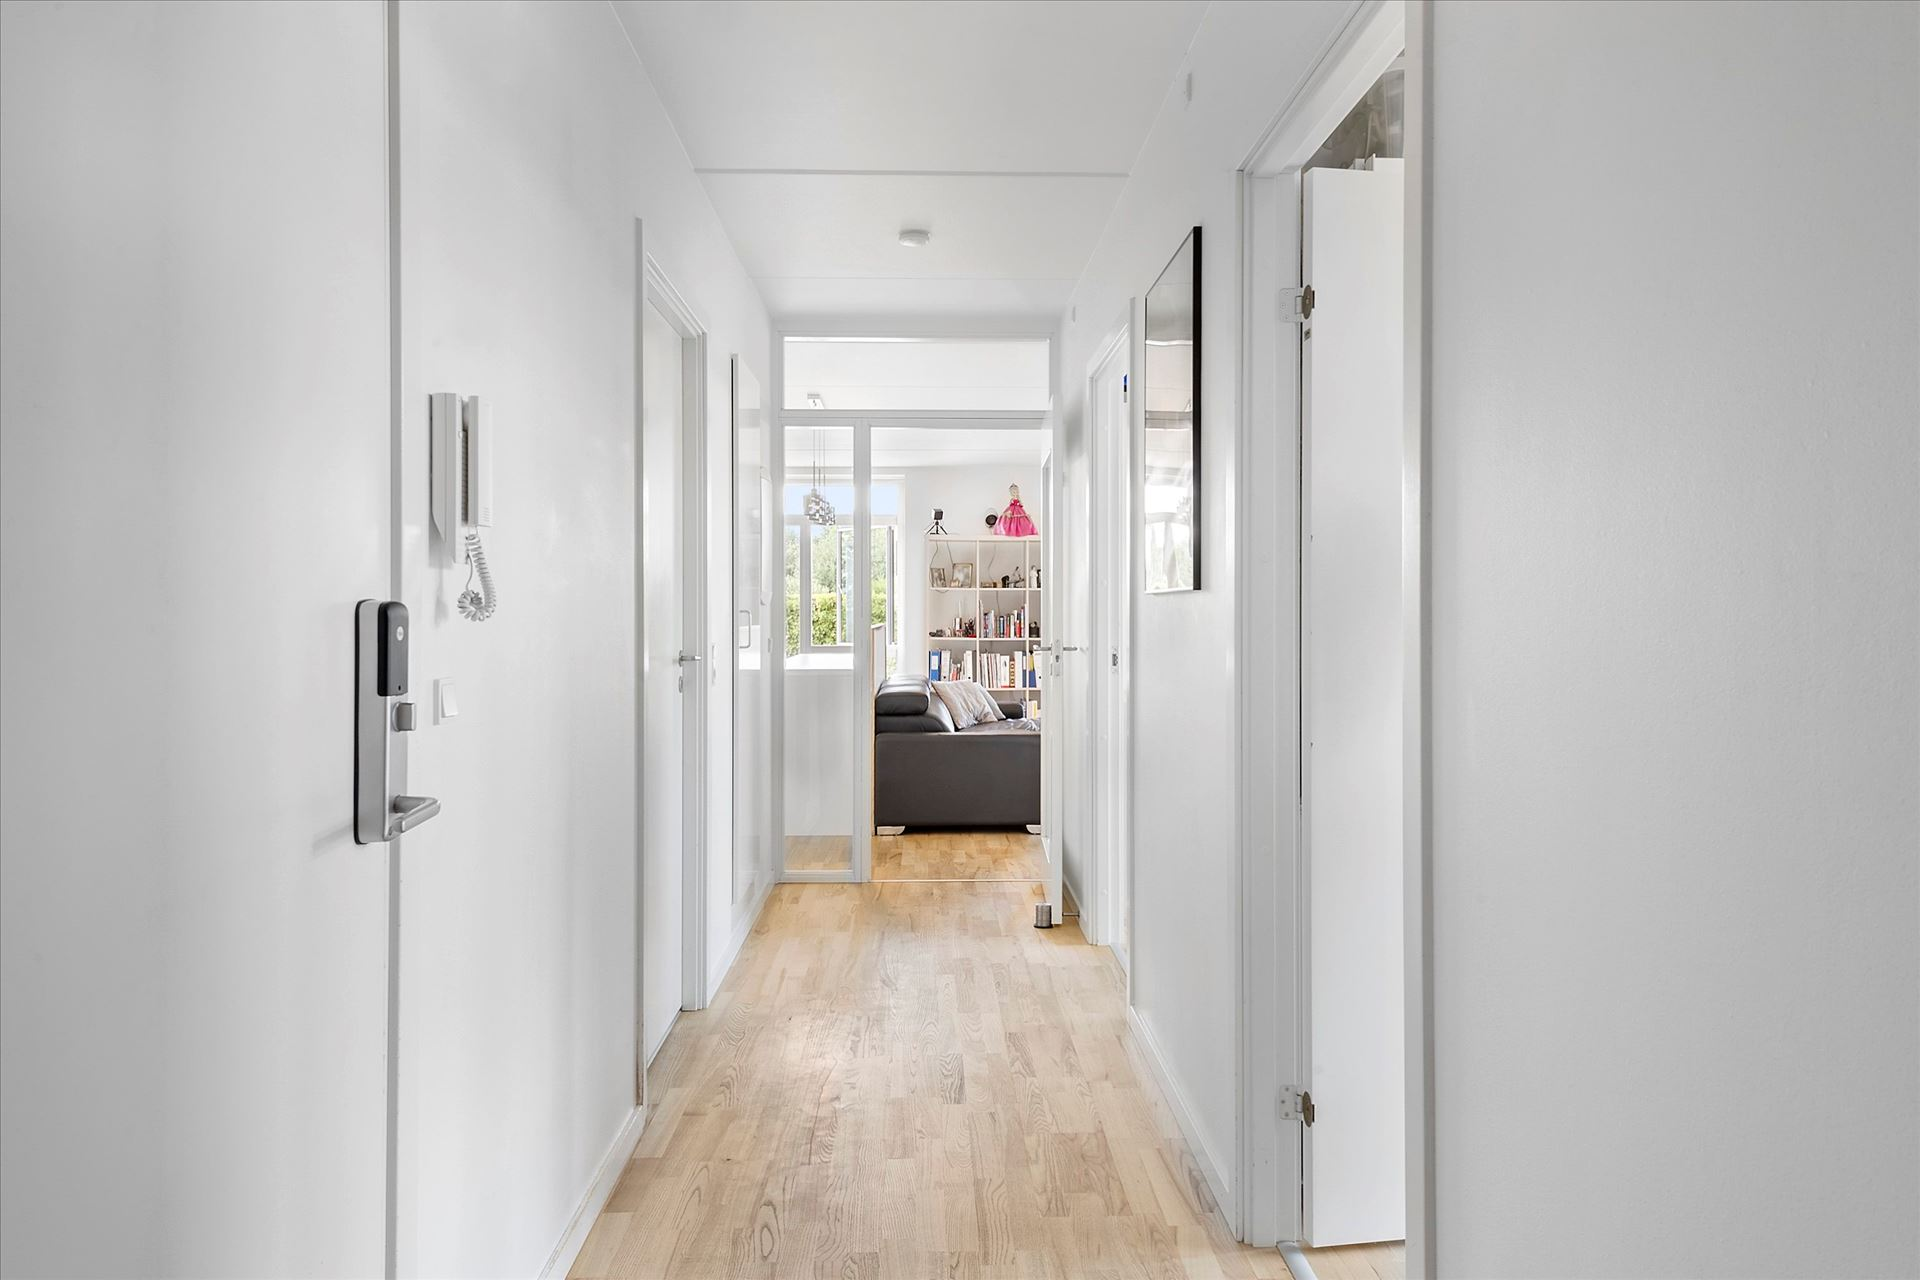
\includegraphics[width=\textwidth]{pictures/random/entre}
      \caption{Label: Entre}
      \label{fig:4}
    \end{subfigure}
    \caption{Sample images from each class}
    \label{fig:misfoster}
\end{figure}
The labeled dataset consists of 6 classes. The labeled dataset is split into a training, validation and testing set, of respectively: 60\% 20\% 20\%.
\begin{table}[H]
    \resizebox{\textwidth}{!}{%
    \begin{tabular}{@{}llllllll@{}}
        \toprule
        \textbf{}           & kitchen       & living\_room & bed\_room    & bath\_room   & dining\_room & entre        & \textbf{total} \\ \midrule
        \textbf{Train}      & 745           & 702          & 622          & 639          & 583          & 541          & \textbf{3842}  \\
        \textbf{Test}       & 256           & 231          & 218          & 210          & 195          & 164          & \textbf{1281}  \\
        \textbf{Validation} & 253           & 239          & 205          & 212          & 194          & 182          & \textbf{1292}  \\ \midrule
        \textbf{Total}      & \textbf{1254} & \textbf{1172} & \textbf{1045} & \textbf{1059} & \textbf{972} & \textbf{887} & \textbf{6415}  \\ \bottomrule
        \end{tabular} %
    }
    \caption{Labeled images from various Danish real-estate pages}
    \label{tab:datadist}
\end{table}
